\documentclass{article}
\usepackage
[
    a4paper,
    top=2cm,
    bottom=3cm,
    left=2cm,
    right=2cm
]{geometry}
\usepackage{amssymb}
\usepackage{amsmath}
\usepackage{amsthm}
\usepackage{mathtools}
\usepackage{array}
\usepackage{xeCJK}
\usepackage{tikz}
\setCJKmainfont{微軟正黑體}
\renewcommand{\thesection}{(\arabic{section})}
\renewcommand{\thesubsection}{(\roman{subsection})}
\newtheorem{lemma}{Lemma}
\newtheorem{corollary}{Corollary}
% \renewcommand{\qedsymbol}{}
\newcommand{\figw}{0.15\paperwidth}
\newcommand{\mg}{\ifmmode \mathcal{G} \else $\mathcal{G}$ \fi}
\newcommand{\fig}[1]{\includegraphics[width=\figw]{fig/#1}}
\newcommand{\OR}{\; | \;}
\newcommand{\set}[1]{ \{ #1 \} }
\newcommand{\Rule}[2][R:]{
\begin{tabular}{c c}
    $#1$ & $#2$ \\
\end{tabular}
}

\title{自動機與形式語言 Homework 3}
\author{Class 02 B03902086 李鈺昇}
\date{}

\begin{document}
    \maketitle
    
    \section{}
        \begin{tabular}{m{\figw}|m{\figw}|m{\figw}|m{\figw}|m{\figw}}
            (i) In \mg & (ii) Not in \mg & (iii) In \mg & (iv) In \mg & (v) In \mg \\
            \fig{i} & The numbers of $a$'s and $b$'s differ. See Corollary 1 in Problem (5). & \fig{iii} & \fig{iv} & \fig{v} \\
        \end{tabular}
        
    \section{}
        \subsection{$\mg = \langle \set{a, b}, \set{S}, R, S \rangle$}
            \Rule{S \rightarrow aS \OR aSb \OR a}
        \subsection{$\mg = \langle \set{a, b}, \set{S}, R, S \rangle$}
            \Rule{S \rightarrow Sb \OR aSb \OR b}
        \subsection{$\mg = \langle \set{a, b}, \set{S}, R, S \rangle$}
            \Rule{S \rightarrow aaSb \OR \epsilon}
        \subsection{$\mg = \langle \set{a, b, \$}, \set{S}, R, S \rangle$}
            \Rule{S \rightarrow aSa \OR bSb \OR \$}
        \subsection{$\mg = \langle \set{a, b}, \set{S, A, B, C}, R, S \rangle$}
            \Rule{S \rightarrow A \OR B \OR bC \OR aCbCaC} \\
            \Rule[\phantom{R:}]{A \rightarrow aA \OR aAb \OR a} \\
            \Rule[\phantom{R:}]{B \rightarrow Bb \OR aBb \OR b} \\
            \Rule[\phantom{R:}]{C \rightarrow aC \OR bC \OR \epsilon}
    
    \section{}
        In the following PDAs, I use $\xrightarrow{a, u, v}$ to mean a transition that reads input $a \in \Sigma \cup \{ \epsilon \}$, pops $u \in \Gamma^*$, and pushes $v \in \Gamma^*$, where the order of popping and pushing is from right to left.
        
        \subsection{}
            \begin{center}
            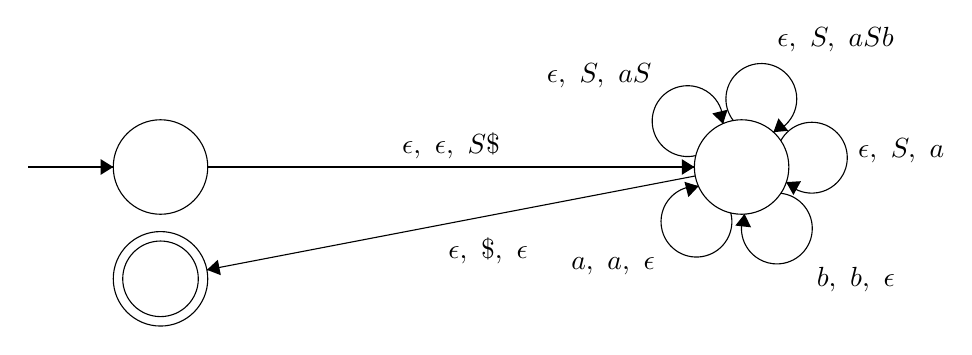
\begin{tikzpicture}[scale=0.2]
            \tikzstyle{every node}+=[inner sep=0pt]
            \draw [black] (18,-26.8) circle (3);
            \draw [black] (54.9,-26.8) circle (3);
            \draw [black] (18,-33.9) circle (3);
            \draw [black] (18,-33.9) circle (2.4);
            \draw [black] (9.6,-26.8) -- (15,-26.8);
            \fill [black] (15,-26.8) -- (14.2,-26.3) -- (14.2,-27.3);
            \draw [black] (21,-26.8) -- (51.9,-26.8);
            \fill [black] (51.9,-26.8) -- (51.1,-26.3) -- (51.1,-27.3);
            \draw (36.45,-26.3) node [above] {$\epsilon,\mbox{ }\epsilon,\mbox{ }S\$$};
            \draw [black] (51.95,-27.37) -- (20.95,-33.33);
            \fill [black] (20.95,-33.33) -- (21.83,-33.67) -- (21.64,-32.69);
            \draw (38.8,-31.24) node [below] {$\epsilon,\mbox{ }\$,\mbox{ }\epsilon$};
            \draw [black] (52.002,-26.072) arc (283.62695:-4.37305:2.25);
            \draw (49.21,-20.98) node [left] {$\epsilon,\mbox{ }S,\mbox{ }aS$};
            \fill [black] (53.72,-24.06) -- (54.01,-23.16) -- (53.04,-23.4);
            \draw [black] (54.376,-23.858) arc (217.82504:-70.17496:2.25);
            \draw (60.87,-19.55) node [above] {$\epsilon,\mbox{ }S,\mbox{ }aSb$};
            \fill [black] (56.92,-24.59) -- (57.86,-24.5) -- (57.24,-23.71);
            \draw [black] (57.383,-25.137) arc (151.53548:-136.46452:2.25);
            \draw (62.27,-25.77) node [right] {$\epsilon,\mbox{ }S,\mbox{ }a$};
            \fill [black] (57.73,-27.76) -- (58.19,-28.58) -- (58.67,-27.7);
            \draw [black] (54.211,-29.708) arc (14.40637:-273.59363:2.25);
            \draw (46.74,-32.49) node [below] {$a,\mbox{ }a,\mbox{ }\epsilon$};
            \fill [black] (52.17,-28.02) -- (51.27,-27.74) -- (51.52,-28.71);
            \draw [black] (57.38,-28.467) arc (83.8351:-204.1649:2.25);
            \draw (62.15,-33.16) node [below] {$b,\mbox{ }b,\mbox{ }\epsilon$};
            \fill [black] (55.09,-29.78) -- (54.5,-30.52) -- (55.5,-30.63);
            \end{tikzpicture}
            \end{center}
        
        \subsection{}
            \begin{center}
            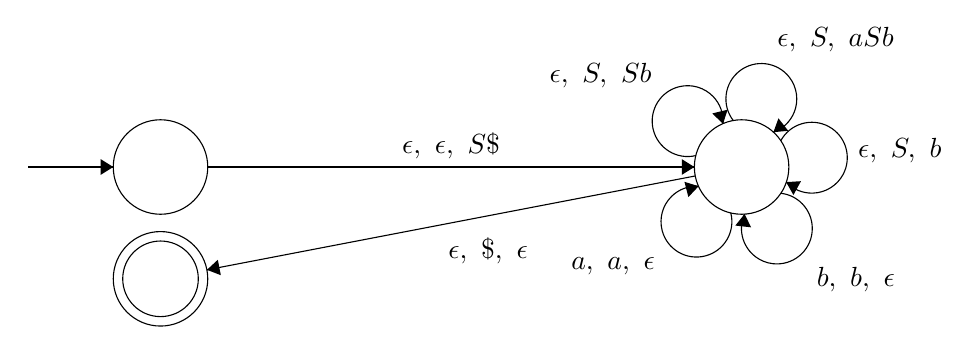
\begin{tikzpicture}[scale=0.2]
            \tikzstyle{every node}+=[inner sep=0pt]
            \draw [black] (18,-26.8) circle (3);
            \draw [black] (54.9,-26.8) circle (3);
            \draw [black] (18,-33.9) circle (3);
            \draw [black] (18,-33.9) circle (2.4);
            \draw [black] (9.6,-26.8) -- (15,-26.8);
            \fill [black] (15,-26.8) -- (14.2,-26.3) -- (14.2,-27.3);
            \draw [black] (21,-26.8) -- (51.9,-26.8);
            \fill [black] (51.9,-26.8) -- (51.1,-26.3) -- (51.1,-27.3);
            \draw (36.45,-26.3) node [above] {$\epsilon,\mbox{ }\epsilon,\mbox{ }S\$$};
            \draw [black] (51.95,-27.37) -- (20.95,-33.33);
            \fill [black] (20.95,-33.33) -- (21.83,-33.67) -- (21.64,-32.69);
            \draw (38.8,-31.24) node [below] {$\epsilon,\mbox{ }\$,\mbox{ }\epsilon$};
            \draw [black] (52.002,-26.072) arc (283.62695:-4.37305:2.25);
            \draw (49.21,-20.98) node [left] {$\epsilon,\mbox{ }S,\mbox{ }Sb$};
            \fill [black] (53.72,-24.06) -- (54.01,-23.16) -- (53.04,-23.4);
            \draw [black] (54.376,-23.858) arc (217.82504:-70.17496:2.25);
            \draw (60.87,-19.55) node [above] {$\epsilon,\mbox{ }S,\mbox{ }aSb$};
            \fill [black] (56.92,-24.59) -- (57.86,-24.5) -- (57.24,-23.71);
            \draw [black] (57.383,-25.137) arc (151.53548:-136.46452:2.25);
            \draw (62.27,-25.77) node [right] {$\epsilon,\mbox{ }S,\mbox{ }b$};
            \fill [black] (57.73,-27.76) -- (58.19,-28.58) -- (58.67,-27.7);
            \draw [black] (54.211,-29.708) arc (14.40637:-273.59363:2.25);
            \draw (46.74,-32.49) node [below] {$a,\mbox{ }a,\mbox{ }\epsilon$};
            \fill [black] (52.17,-28.02) -- (51.27,-27.74) -- (51.52,-28.71);
            \draw [black] (57.38,-28.467) arc (83.8351:-204.1649:2.25);
            \draw (62.15,-33.16) node [below] {$b,\mbox{ }b,\mbox{ }\epsilon$};
            \fill [black] (55.09,-29.78) -- (54.5,-30.52) -- (55.5,-30.63);
            \end{tikzpicture}
            \end{center}
        
        \subsection{}
            \begin{center}
            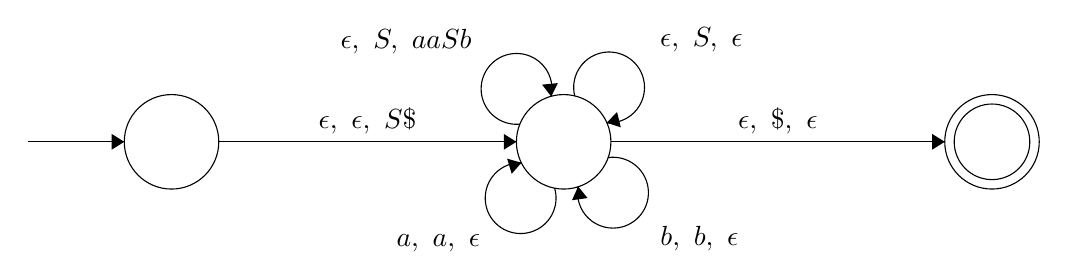
\begin{tikzpicture}[scale=0.2]
            \tikzstyle{every node}+=[inner sep=0pt]
            \draw [black] (40.6,-28) circle (3);
            \draw [black] (67.8,-28) circle (3);
            \draw [black] (67.8,-28) circle (2.4);
            \draw [black] (15.7,-28) circle (3);
            \draw [black] (43.6,-28) -- (64.8,-28);
            \fill [black] (64.8,-28) -- (64,-27.5) -- (64,-28.5);
            \draw (54.2,-27.5) node [above] {$\epsilon,\mbox{ }\$,\mbox{ }\epsilon$};
            \draw [black] (37.831,-26.877) arc (275.66544:-12.33456:2.25);
            \draw (30.59,-22.47) node [above] {$\epsilon,\mbox{ }S,\mbox{ }aaSb$};
            \fill [black] (39.81,-25.12) -- (40.23,-24.27) -- (39.23,-24.37);
            \draw [black] (41.304,-25.096) arc (194.11294:-93.88706:2.25);
            \draw (49.35,-22.33) node [above] {$\epsilon,\mbox{ }S,\mbox{ }\epsilon$};
            \fill [black] (43.33,-26.79) -- (44.23,-27.08) -- (43.99,-26.11);
            \draw [black] (40.023,-30.932) arc (16.601:-271.399:2.25);
            \draw (32.64,-33.86) node [below] {$a,\mbox{ }a,\mbox{ }\epsilon$};
            \fill [black] (37.92,-29.33) -- (37.01,-29.07) -- (37.3,-30.03);
            \draw [black] (43.415,-29.003) arc (98.12244:-189.87756:2.25);
            \draw (49.22,-33.33) node [below] {$b,\mbox{ }b,\mbox{ }\epsilon$};
            \fill [black] (41.52,-30.84) -- (41.13,-31.71) -- (42.12,-31.57);
            \draw [black] (6.6,-28) -- (12.7,-28);
            \fill [black] (12.7,-28) -- (11.9,-27.5) -- (11.9,-28.5);
            \draw [black] (18.7,-28) -- (37.6,-28);
            \fill [black] (37.6,-28) -- (36.8,-27.5) -- (36.8,-28.5);
            \draw (28.15,-27.5) node [above] {$\epsilon,\mbox{ }\epsilon,\mbox{ }S\$$};
            \end{tikzpicture}
            \end{center}
        
        \subsection{}
            \begin{center}
            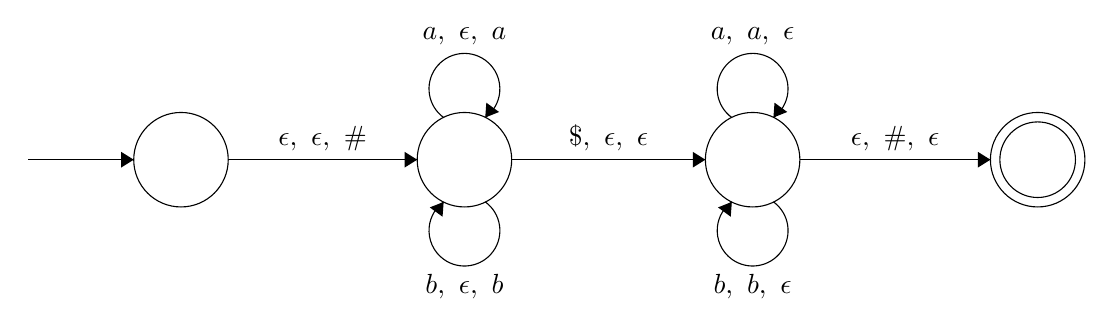
\begin{tikzpicture}[scale=0.2]
            \tikzstyle{every node}+=[inner sep=0pt]
            \draw [black] (14.2,-29.9) circle (3);
            \draw [black] (32.2,-29.9) circle (3);
            \draw [black] (50.5,-29.9) circle (3);
            \draw [black] (68.6,-29.9) circle (3);
            \draw [black] (68.6,-29.9) circle (2.4);
            \draw [black] (4.5,-29.9) -- (11.2,-29.9);
            \fill [black] (11.2,-29.9) -- (10.4,-29.4) -- (10.4,-30.4);
            \draw [black] (17.2,-29.9) -- (29.2,-29.9);
            \fill [black] (29.2,-29.9) -- (28.4,-29.4) -- (28.4,-30.4);
            \draw (23.2,-29.4) node [above] {$\epsilon,\mbox{ }\epsilon,\mbox{ }\#$};
            \draw [black] (35.2,-29.9) -- (47.5,-29.9);
            \fill [black] (47.5,-29.9) -- (46.7,-29.4) -- (46.7,-30.4);
            \draw (41.35,-29.4) node [above] {$\$,\mbox{ }\epsilon,\mbox{ }\epsilon$};
            \draw [black] (53.5,-29.9) -- (65.6,-29.9);
            \fill [black] (65.6,-29.9) -- (64.8,-29.4) -- (64.8,-30.4);
            \draw (59.55,-29.4) node [above] {$\epsilon,\mbox{ }\#,\mbox{ }\epsilon$};
            \draw [black] (49.177,-27.22) arc (234:-54:2.25);
            \draw (50.5,-22.65) node [above] {$a,\mbox{ }a,\mbox{ }\epsilon$};
            \fill [black] (51.82,-27.22) -- (52.7,-26.87) -- (51.89,-26.28);
            \draw [black] (51.823,-32.58) arc (54:-234:2.25);
            \draw (50.5,-37.15) node [below] {$b,\mbox{ }b,\mbox{ }\epsilon$};
            \fill [black] (49.18,-32.58) -- (48.3,-32.93) -- (49.11,-33.52);
            \draw [black] (30.877,-27.22) arc (234:-54:2.25);
            \draw (32.2,-22.65) node [above] {$a,\mbox{ }\epsilon,\mbox{ }a$};
            \fill [black] (33.52,-27.22) -- (34.4,-26.87) -- (33.59,-26.28);
            \draw [black] (33.523,-32.58) arc (54:-234:2.25);
            \draw (32.2,-37.15) node [below] {$b,\mbox{ }\epsilon,\mbox{ }b$};
            \fill [black] (30.88,-32.58) -- (30,-32.93) -- (30.81,-33.52);
            \end{tikzpicture}
            \end{center}
        
        \subsection{}
            \begin{center}
            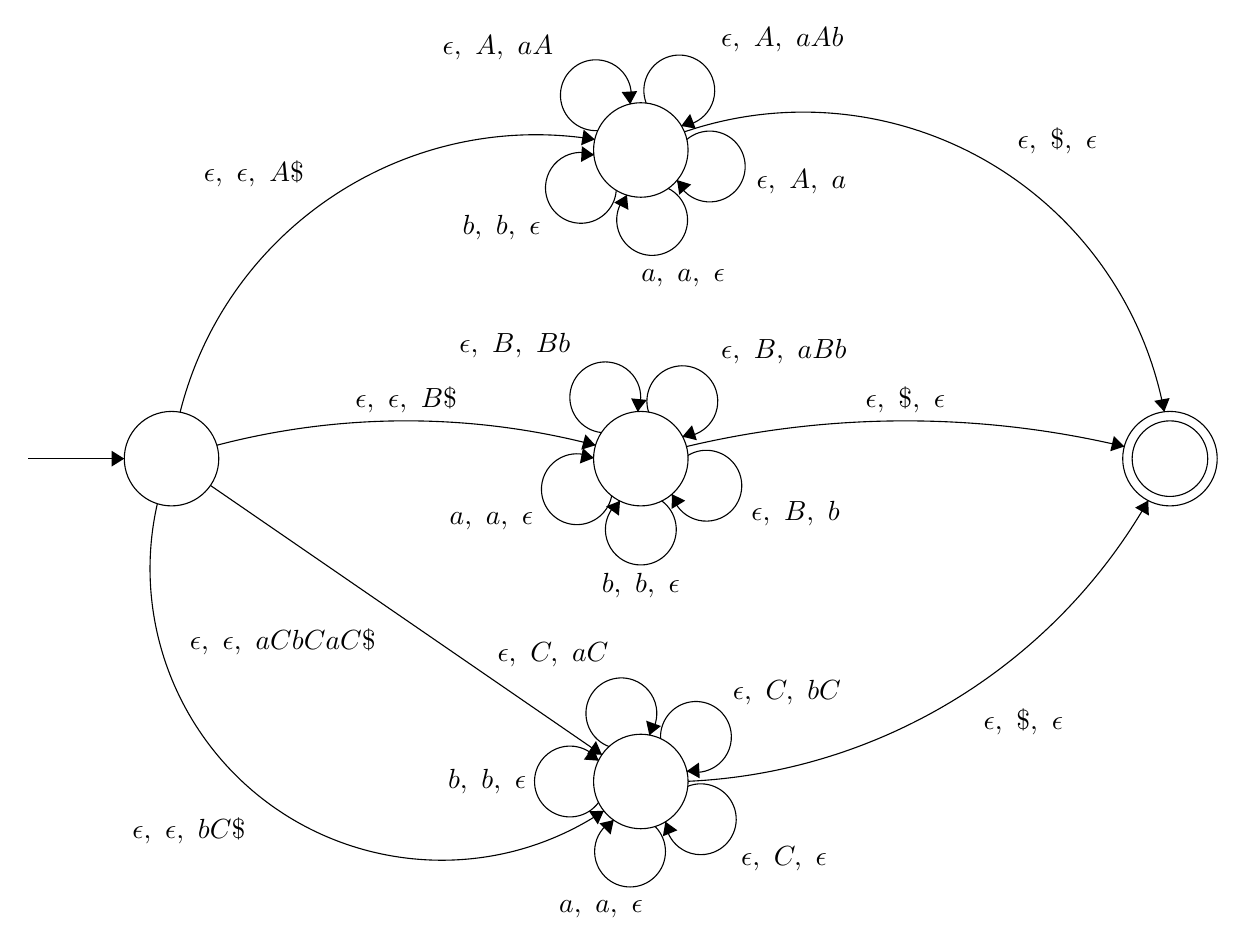
\begin{tikzpicture}[scale=0.2]
            \tikzstyle{every node}+=[inner sep=0pt]
            \draw [black] (41.2,-28.4) circle (3);
            \draw [black] (74.8,-28.4) circle (3);
            \draw [black] (74.8,-28.4) circle (2.4);
            \draw [black] (41.2,-8.8) circle (3);
            \draw [black] (11.4,-28.4) circle (3);
            \draw [black] (41.2,-48.9) circle (3);
            \draw [black] (44.1,-27.632) arc (103.39726:76.60274:59.992);
            \fill [black] (71.9,-27.63) -- (71.24,-26.96) -- (71.01,-27.93);
            \draw (58,-25.5) node [above] {$\epsilon,\mbox{ }\$,\mbox{ }\epsilon$};
            \draw [black] (38.712,-26.745) arc (264.10644:-23.89356:2.25);
            \draw (33.2,-22.05) node [above] {$\epsilon,\mbox{ }B,\mbox{ }Bb$};
            \fill [black] (41,-25.42) -- (41.58,-24.67) -- (40.58,-24.57);
            \draw [black] (41.698,-25.454) arc (198.13823:-89.86177:2.25);
            \draw (50.28,-22.43) node [above] {$\epsilon,\mbox{ }B,\mbox{ }aBb$};
            \fill [black] (43.84,-27) -- (44.76,-27.23) -- (44.45,-26.28);
            \draw [black] (44.182,-28.201) arc (121.55195:-166.44805:2.25);
            \draw (48.18,-31.89) node [right] {$\epsilon,\mbox{ }B,\mbox{ }b$};
            \fill [black] (43.17,-30.65) -- (43.16,-31.59) -- (44.02,-31.07);
            \draw [black] (39.352,-30.749) arc (-10.46138:-298.46138:2.25);
            \draw (34.4,-32.37) node [left] {$a,\mbox{ }a,\mbox{ }\epsilon$};
            \fill [black] (38.21,-28.36) -- (37.52,-27.73) -- (37.33,-28.71);
            \draw [black] (42.523,-31.08) arc (54:-234:2.25);
            \draw (41.2,-35.65) node [below] {$b,\mbox{ }b,\mbox{ }\epsilon$};
            \fill [black] (39.88,-31.08) -- (39,-31.43) -- (39.81,-32.02);
            \draw [black] (38.478,-7.568) arc (273.37707:-14.62293:2.25);
            \draw (32.12,-3.09) node [above] {$\epsilon,\mbox{ }A,\mbox{ }aA$};
            \fill [black] (40.52,-5.89) -- (40.97,-5.06) -- (39.98,-5.12);
            \draw [black] (43.968,-7.649) arc (108.88325:10.60388:23.321);
            \fill [black] (74.44,-25.42) -- (74.78,-24.55) -- (73.8,-24.73);
            \draw (67.65,-9.07) node [above] {$\epsilon,\mbox{ }\$,\mbox{ }\epsilon$};
            \draw [black] (41.544,-5.832) arc (201.11673:-86.88327:2.25);
            \draw (50.18,-2.63) node [above] {$\epsilon,\mbox{ }A,\mbox{ }aAb$};
            \fill [black] (43.77,-7.27) -- (44.69,-7.45) -- (44.33,-6.51);
            \draw [black] (44.114,-8.138) arc (130.52889:-157.47111:2.25);
            \draw (48.52,-10.8) node [right] {$\epsilon,\mbox{ }A,\mbox{ }a$};
            \fill [black] (43.5,-10.71) -- (43.64,-11.64) -- (44.4,-10.99);
            \draw [black] (42.933,-11.235) arc (63.16759:-224.83241:2.25);
            \draw (43.88,-16.33) node [below] {$a,\mbox{ }a,\mbox{ }\epsilon$};
            \fill [black] (40.32,-11.66) -- (39.51,-12.14) -- (40.41,-12.6);
            \draw [black] (39.641,-11.349) arc (-3.72436:-291.72436:2.25);
            \draw (34.87,-13.7) node [left] {$b,\mbox{ }b,\mbox{ }\epsilon$};
            \fill [black] (38.23,-9.11) -- (37.46,-8.56) -- (37.4,-9.56);
            \draw [black] (13.87,-30.1) -- (38.73,-47.2);
            \fill [black] (38.73,-47.2) -- (38.35,-46.33) -- (37.79,-47.16);
            \draw (18.47,-39.15) node [below] {$\epsilon,\mbox{ }\epsilon,\mbox{ }aCbCaC\$$};
            \draw [black] (39.193,-46.686) arc (249.92849:-38.07151:2.25);
            \draw (35.62,-41.65) node [above] {$\epsilon,\mbox{ }C,\mbox{ }aC$};
            \fill [black] (41.74,-45.96) -- (42.48,-45.38) -- (41.54,-45.04);
            \draw [black] (42.453,-46.187) arc (182.95198:-105.04802:2.25);
            \draw (47.01,-43.23) node [right] {$\epsilon,\mbox{ }C,\mbox{ }bC$};
            \fill [black] (44.12,-48.24) -- (44.94,-48.7) -- (44.89,-47.7);
            \draw [black] (44.172,-49.209) arc (111.79915:-176.20085:2.25);
            \draw (47.54,-53.79) node [right] {$\epsilon,\mbox{ }C,\mbox{ }\epsilon$};
            \fill [black] (42.76,-51.45) -- (42.6,-52.38) -- (43.52,-52);
            \draw [black] (42.099,-51.75) arc (45.24216:-242.75784:2.25);
            \draw (38.67,-56.43) node [below] {$a,\mbox{ }a,\mbox{ }\epsilon$};
            \fill [black] (39.48,-51.35) -- (38.57,-51.56) -- (39.28,-52.27);
            \draw [black] (38.52,-50.223) arc (324:36:2.25);
            \draw (33.95,-48.9) node [left] {$b,\mbox{ }b,\mbox{ }\epsilon$};
            \fill [black] (38.52,-47.58) -- (38.17,-46.7) -- (37.58,-47.51);
            \draw [black] (73.419,-31.062) arc (-29.82929:-87.39438:35.545);
            \fill [black] (73.42,-31.06) -- (72.59,-31.51) -- (73.46,-32.01);
            \draw (65.49,-44.23) node [below] {$\epsilon,\mbox{ }\$,\mbox{ }\epsilon$};
            \draw [black] (2.3,-28.4) -- (8.4,-28.4);
            \fill [black] (8.4,-28.4) -- (7.6,-27.9) -- (7.6,-28.9);
            \draw [black] (14.276,-27.548) arc (104.68841:75.31159:47.42);
            \fill [black] (38.32,-27.55) -- (37.68,-26.86) -- (37.42,-27.83);
            \draw (26.3,-25.5) node [above] {$\epsilon,\mbox{ }\epsilon,\mbox{ }B\$$};
            \draw [black] (11.944,-25.452) arc (165.85989:80.8074:23.315);
            \fill [black] (38.28,-8.13) -- (37.57,-7.51) -- (37.41,-8.5);
            \draw (16.63,-11.17) node [above] {$\epsilon,\mbox{ }\epsilon,\mbox{ }A\$$};
            \draw [black] (38.854,-50.764) arc (-56.17174:-192.87794:18.514);
            \fill [black] (38.85,-50.76) -- (37.91,-50.79) -- (38.47,-51.63);
            \draw (12.5,-51.14) node [below] {$\epsilon,\mbox{ }\epsilon,\mbox{ }bC\$$};
            \end{tikzpicture}
            \end{center}
        
    \section{}
        \subsection{}
            Suppose $L_1$ is a CFL, and the pumping length is $p$. Take $u = a^p b^p c^p \in L_1$. Clearly $|u| = 3p \geq p$, and pumping lemma ensures the existence of $s, x, y, z, t \in \{a, b, c\}^*$ such that $u = sxyzt, |xz| > 0, s x^i y z^i t \in L_1 \; \forall i \geq 0$. \\
            If either $x$ or $z$ contains at least two kinds of symbols, $s x^2 y z^2 t$ will not be in the form $a^* b^* c^*$, hence not in $L_1$. \\
            On the other hand, if $x$ and $z$ each contains at most one kind of symbol, then at most two kinds of symbols appear in $xz$. We can check the three possible cases:
            \begin{itemize}
                \item There is no $a$ in $xz$ \\
                    $s x^0 y z^0 t \notin L_1$ since it has the same number of $a$ but fewer $b$ or fewer $c$.
                \item There is no $b$ in $xz$ \\
                    If there is $a$ in $xz$, then $s x^2 y z^2 t \notin L_1$ since it has the same number of $b$ but more $a$. Otherwise there is $c$ in $xz$ (since $|xz| > 0$), then $s x^0 y z^0 t \notin L_1$ since it has the same number of $b$ but fewer $c$.
                \item There is no $c$ in $xz$ \\
                    $s x^2 y z^2 t \notin L_1$ since it has the same number of $c$ but fewer $a$ or fewer $b$.
            \end{itemize}
            In either case, $u$ can't be pumped, violating the pumping lemma. Thus $L_1$ is not a CFL.
        
        \subsection{}
            Suppose $L_2$ is a CFL, and the pumping length is $p$. Take $u = a^p b^{2p} c^{3p} \in L_2$. Clearly $|u| = 6p \geq p$, and pumping lemma ensures the existence of $s, x, y, z, t \in \{a, b, c\}^*$ such that $u = sxyzt, |xz| > 0, s x^i y z^i t \in L_2 \; \forall i \geq 0$. \\
            If either $x$ or $z$ contains at least two kinds of symbols, $s x^2 y z^2 t$ will not be in the form $a^* b^* c^*$, hence not in $L_2$. \\
            On the other hand, if $x$ and $z$ each contains at most one kind of symbol, then at most two kinds of symbols appear in $xz$. It's clear that we need to add $k$ $a$, $2k$ $b$, $3k$ $c$ simultaneously to maintain the $1:2:3$ ratio. But $s x^2 y z^2 t$ adds at most two kinds of symbols, so $s x^2 y z^2 t \notin L_2$. \\
            In either case, $u$ can't be pumped, violating the pumping lemma. Thus $L_2$ is not a CFL.
        
        \subsection{}
            Suppose $L_3$ is a CFL, and the pumping length is $p$. Pick any prime $q \geq p$. Take $u = a^q \in L_3$. Clearly $|u| = q \geq p$, and pumping lemma ensures the existence of $s, x, y, z, t \in a^*$ such that $u = sxyzt, |xz| > 0, s x^i y z^i t \in L_3 \; \forall i \geq 0$. \\
            We examine $v = s x^{q+1} y z^{q+1} t$, whose length $|v| = |sxyzt| + |x^q z^q| = q + q|xz| = q(|xz| + 1)$. Since $|xz| > 0$, we have $|xz| + 1 \geq 2$, and so $|v|$ is not a prime. Hence $v \notin L_3$, $u$ can't be pumped, violating the pumping lemma. Thus $L_3$ is not a CFL.
    
    \section{}
        For $w \in \set{a, b, S}^*$, define $\alpha(w)$ to be the number of $a$'s in $w$, and $\beta(w)$ to be the number of $b$'s in $w$. Let $L = \set{w \in \set{a, b}^* \OR \alpha(w) = \beta(w)}$. \\
        The desired equality $L = L(\mg)$ is proved by the following two lemmas.
        
        \begin{lemma}
            $L(\mg) \subseteq L$
        \end{lemma}
        
        \begin{proof}
            For the CFG \mg, name $S \rightarrow SS \OR \epsilon$ as Rule 1 and $S \rightarrow aSb \OR bSa$ as Rule 2 (each of Rule 1 and Rule 2 has two rules). \\
            I shall show that for any $w \in L(\mg)$, $\alpha(w) = \beta(w)$. Because $w \in L(\mg)$, there is a derivation $S \overset{*}{\implies} w$. Starting from the start variable $S$, $\alpha(S) = \beta(S) = 0$. Next consider each rule applied for $u \implies v$, given $\alpha(u) = \beta(u)$.
            \begin{itemize}
                \item The rule belongs to Rule 1 \\
                    One $S$ is replaced with either $SS$ or $\epsilon$, adding no $a$ or $b$. So $\alpha(v) = \alpha(u)$ and $\beta(v) = \beta(u)$. Thus $\alpha(v) = \beta(v)$.
                \item The rule belongs to Rule 2 \\
                    One $S$ is replaced with either $aSb$ or $bSa$, adding one $a$ and one $b$. So $\alpha(v) = \alpha(u) + 1$ and $\beta(v) = \beta(u) + 1$. Thus $\alpha(v) = \beta(v)$.
            \end{itemize}
            In either case, the equation $\alpha(\cdot) = \beta(\cdot)$ is maintained after applying the rule. So we can conclude that $\alpha(w) = \beta(w)$.
        \end{proof}
        
        \begin{corollary}
            If $w \in \set{a, b}^*$ contains different numbers of $a$'s and $b$'s, then $w \notin L(\mg)$. 
        \end{corollary}
        
        ~ \\
        
        \begin{lemma}
            $L \subseteq L(\mg)$
        \end{lemma}
        
        \begin{proof}
            I shall show that for any $w \in L$, $w \in L(\mg)$. Let's prove it by induction on $\alpha(w)$.
            \begin{itemize}
                \item Basis: $w \in L, \alpha(w) = 0$. Then $\beta(w) = 0$, and thus $w = \epsilon$. Using the rule $S \rightarrow \epsilon$, we have the derivation $S \implies \epsilon$, hence $w \in L(\mg)$. So the lemma holds for $\alpha(w) = 0$.
                \item Induction hypothesis: Suppose the lemma holds for $w$ with $\alpha(w) \leq n$, for some $n \geq 0$.
                \item Induction step: For any $w \in L$ with $\alpha(w) = n + 1$, we know $\beta(w) = n + 1$, implying $|w| = 2n + 2$. Write $w = w_0 w_1 \cdots w_{2n} w_{2n+1}$. Consider $w_0$ and $w_{2n+1}$:
                \begin{itemize}
                    \item $w_0 \neq w_{2n+1}$ \\
                        Let $w' = w_1 \cdots w_{2n}$ so that $w = w_0 w' w_{2n+1}$. Because $w_0 \neq w_{2n+1}$, it's obvious $\alpha(w') = \beta(w') = n$.
                        By the induction hypothesis, there is a derivation $S \overset{*}{\implies} w'$. \\
                        Now if $w_0 = a, w_{2n+1} = b$, then $S \implies aSb \overset{*}{\implies} aw'b = w$.
                        Otherwise, $w_0 = b, w_{2n+1} = a$, and $S \implies bSa \overset{*}{\implies} bw'a = w$.
                    \item $w_0 = w_{2n+1}$ \\
                        Define a function $f(i) \equiv \alpha(w_0 \cdots w_i) - \beta(w_0 \cdots w_i)$ for $0 \leq i \leq 2n+1$.
                        Because $w_0 \cdots w_i$ and $w_0 \cdots w_{i+1}$ differs only by a single $a$ or a single $b$, only $\alpha(\cdot)$ or $\beta(\cdot)$ differs by $\pm 1$.
                        So we know $f(i+1) - f(i) = \pm 1$ for $0 \leq i \leq 2n$. \\
                        Because $\alpha(w) = \beta(w)$, $f(2n+1) = 0$.
                        Now if $w_0 = w_{2n+1} = a$, then $f(0) = 1$ and $f(2n) = -1$.
                        Otherwise, $w_0 = w_{2n+1} = b$, then $f(0) = -1$ and $f(2n) = 1$.
                        In either case, $f(0)f(2n) = -1 < 0$, so there must be some $j$ such that $0 < j < 2n$ and $f(j) = 0$ (like the discrete version Intermediate Value Theorem). \\
                        Let $u = w_0 \cdots w_j, v = w_{j+1} \cdots w_{2n+1}$, so that $w = uv$.
                        It's obvious that $2 \leq |u|, |v| \leq 2n$ by $0 < j < 2n$. Because $f(j) = f(2n+1) = 0$, we know $\alpha(u) = \beta(u)$ and $\alpha(v) = \beta(v)$.
                        By the induction hypothesis, $u, v \in L(\mg)$, and thus there are derivations $S \overset{*}{\implies} u$ and $S \overset{*}{\implies} v$.
                        So we can derive $w$ by $S \implies SS \overset{*}{\implies} uS \overset{*}{\implies} uv = w$.
                \end{itemize}
                In either case, there is a derivation from $S$ to $w$, so $w \in L(\mg)$.
            \end{itemize}
            The proof is done by induction.
        \end{proof}
        
        % , so in order to have the derivation $S \overset{*}{\implies} \epsilon$, 
    % $\overset{*}{\implies}$
\end{document}